\setlength{\columnsep}{1cm}

\begin{multicols}{2}
	Тестируемый NOR-элемент должен соответствовать следующей таблице истинности.

	Временная диаграмма на Рисунке 4 показывает изменение напряжений на входах \( A \), \( B \) и выходе \( \text{Out} \) во времени, подтверждая правильность работы NOR-элемента.

	\columnbreak

	\noindent
	\renewcommand{\arraystretch}{1.33}
	\raggedright
	\begin{tabular}{|>{\centering\arraybackslash}p{1.2cm}|>{\centering\arraybackslash}p{1.2cm}|>{\centering\arraybackslash}p{1.6cm}|}
		\hline
		A & B & Out \\
		\hline
		0 & 0 & 1   \\
		0 & 1 & 0   \\
		1 & 0 & 0   \\
		1 & 1 & 0   \\
		\hline
	\end{tabular}

\end{multicols}

\begin{figure}[H]
	\centering
	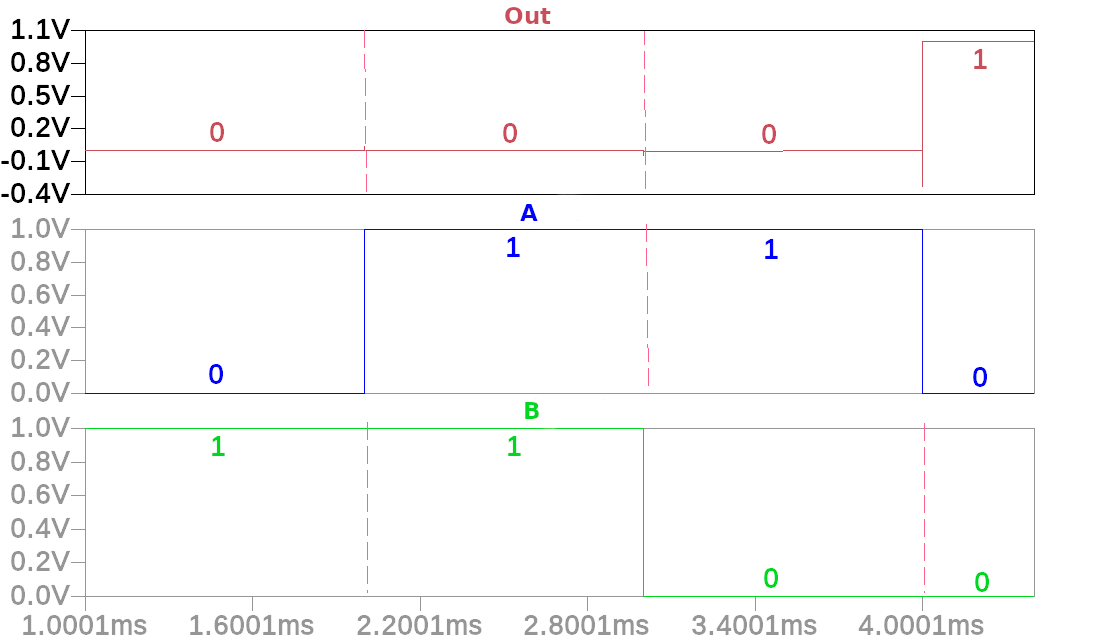
\includegraphics[width=0.8\textwidth]{../data/test_cmos_nor_time}
	\caption{Временная диаграмма напряжений на A, B, Out}
\end{figure}
